%------------------------------------------------------------------------------
% Author(s):
% Varaun Ramgoolie
%
% Copyright:
%  Copyright (C) 2020 Brad Bachu, Arjun Mohammed, Varaun Ramgoolie, Nicholas Sammy
%
%  This file is part of Applied-Mathematics-Unit2 and is distributed under the
%  terms of the MIT License. See the LICENSE file for details.
%
%  Description:
%     Year: 2010  graph for q5 (showing values of t) 
%     Module: 3
%     Question: 5
%------------------------------------------------------------------------------
\documentclass[crop,tikz]{standalone}
\usepackage{pgfplots}
\usepackage{../../../../src/tikzappmath}
\usetikzlibrary{patterns}

\begin{document}
	
	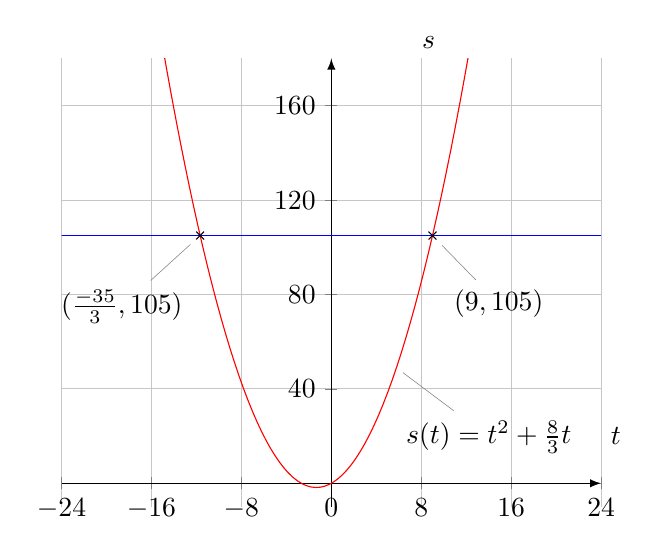
\begin{tikzpicture}
		
		\begin{axis}
			[
			xmin=-24,xmax=24,
			ymin=-10,ymax=180,
			grid=both,
			grid style={line width=0pt, draw=darkgray!10},
			major grid style={line width=0pt,draw=darkgray!30},
			axis lines=left,
			minor tick num=0,
			enlargelimits={abs=0},
			axis line style={-latex},
			axis x line shift=-10,
			axis y line shift=-24,
			samples=1,
			domain = -60:60,
			ytick={40,80,...,160},
			xtick={-24,-16,...,24},
			xlabel={$t$},
			ylabel={$s$},
			x label style={at={(axis description cs:1,0.2)},anchor=north west},
			y label style={at={(axis description cs:0.65,1)},anchor=south west, rotate=-90}
			]
			
			
			\addplot [domain=-60:60, samples=300, color=red]{x^2+2.666666666*x};

			\addplot [domain=-60:60, samples=300, color=blue]{105};
			
			\addplot [mark=x] coordinates {(9,105)} ;

			\addplot [mark=x] coordinates {(-35/3,105)} ;
						
			\node [pin=-100.5:{$(\frac{-35}{3},105)$}] at (axis cs:(-35/3,105) {};
			
			\node [pin=-75:{$(9,105)$}] at (axis cs:(9,105) {};
			
			\node [pin=-86:{$s(t)=t^2+\frac{8}{3}t$}] at (axis cs:(5.5,50) {};
			
		\end{axis}	
		
	\end{tikzpicture}
	
\end{document}